% Compile with XeLaTeX or LuaLaTeX
\documentclass[12pt]{article}
\usepackage[tmargin=1in,bmargin=1in,lmargin=1.25in,rmargin=1.25in]{geometry}
\usepackage{fontspec}
\usepackage{xcolor}
\usepackage{titlesec}
\usepackage{listings}
\usepackage{color}
%\usepackage[latin2]{inputenc}
\usepackage{url}

\definecolor{mygreen}{rgb}{0,0.6,0}
\definecolor{mygray}{rgb}{0.5,0.5,0.5}
\definecolor{mymauve}{rgb}{0.58,0,0.82}

\lstset{ %
  backgroundcolor=\color{white},   % choose the background color; you must add \usepackage{color} or \usepackage{xcolor}
  basicstyle=\footnotesize,        % the size of the fonts that are used for the code
  breakatwhitespace=false,         % sets if automatic breaks should only happen at whitespace
  breaklines=true,                 % sets automatic line breaking
  captionpos=b,                    % sets the caption-position to bottom
  commentstyle=\color{mygreen},    % comment style
  deletekeywords={...},            % if you want to delete keywords from the given language
  escapeinside={\%*}{*)},          % if you want to add LaTeX within your code
  extendedchars=true,              % lets you use non-ASCII characters; for 8-bits encodings only, does not work with UTF-8
  frame=single,                    % adds a frame around the code
  keepspaces=true,                 % keeps spaces in text, useful for keeping indentation of code (possibly needs columns=flexible)
  keywordstyle=\color{blue},       % keyword style
  language=R,                      % the language of the code
  otherkeywords={*,...},           % if you want to add more keywords to the set
  numbers=left,                    % where to put the line-numbers; possible values are (none, left, right)
  numbersep=5pt,                   % how far the line-numbers are from the code
  numberstyle=\tiny\color{mygray}, % the style that is used for the line-numbers
  rulecolor=\color{black},         % if not set, the frame-color may be changed on line-breaks within not-black text (e.g. comments (green here))
  showspaces=false,                % show spaces everywhere adding particular underscores; it overrides 'showstringspaces'
  showstringspaces=false,          % underline spaces within strings only
  showtabs=false,                  % show tabs within strings adding particular underscores
  stepnumber=1,                    % the step between two line-numbers. If it's 1, each line will be numbered
  stringstyle=\color{mymauve},     % string literal style
  tabsize=2,                       % sets default tabsize to 2 spaces
  texcl=true,
  title=\lstname,                  % show the filename of files included with \lstinputlisting; also try caption instead of title
  %inputencoding=utf8,
  %extendedchars=true,
  %literate={á}{{\'a}}1 {{Á}{{\'A}}1 é}{{\'e}}1 {š}{{\~s}}1
}

\defaultfontfeatures{Ligatures=TeX}
% Set sans serif font to Calibri
%\setsansfont{Calibri}
% Set serifed font to Cambria
%\setmainfont{Cambria}
% Define light and dark Microsoft blue colours
\definecolor{MSBlue}{rgb}{.204,.353,.541}
\definecolor{MSLightBlue}{rgb}{.31,.506,.741}
% Define a new fontfamily for the subsubsection font
% Don't use \fontspec directly to change the font
\newfontfamily\subsubsectionfont[Color=MSLightBlue]{Times New Roman}
% Set formats for each heading level
\titleformat*{\section}{\Large\bfseries\sffamily\color{MSBlue}}
\titleformat*{\subsection}{\normalsize\bfseries\sffamily\color{MSLightBlue}}
\titleformat*{\subsubsection}{\small\sffamily\subsubsectionfont}

\begin{document}
\sffamily\fontsize{26}{15}\color{MSBlue}\textbf{MI-SPI 2015 - Domácí úkol č.1}\\
\color{MSBlue}\underline{\hspace{17cm}}
\sffamily\fontsize{12}{15}\color{MSBlue}\textit{Vedoucí týmu: Tomáš Nesrovnal (nesrotom, 107)}\\
\sffamily\fontsize{12}{15}\color{MSBlue}\textit{Členové týmu: Vojtěch Krákora (krakovoj, 103), Tomáš Šabata (sabattom, 103)}\\
\sffamily\fontsize{12}{15}\color{MSBlue}\textit{Datum: 22.4.2015}\\
  \begin{lstlisting}[frame=single]  % Start your code-block

K = nchar('Tomas') # jmeno
L = nchar('Nesrovnal') # prijmeni
\end{lstlisting}
\section{Generování náhodného výběru a grafické ověřování jeho rozdělení:}
\subsection{Generování náhodného výběru}
\begin{footnotesize}
\color{black}
Vygenerovali jsme n náhodných hodnot z exponencionálního rozdělení pomocí inverzní distribuční funkce \cite{wiki}.
\end{footnotesize}

  \begin{lstlisting}[frame=single]  % Start your code-block
  
n = K*20
u=runif(n, min=0, max=1) # Generuje n náhodných hodnot z UNIF(0,1)
x=-log(1-u)/L # Exp rozdelení z rovnomerného inverzní distr. fcí.
\end{lstlisting}
%%%%%%%%%%%%%%%%%%%%%%%%%%%%%%%%%%%%%%%%%%%%%%%%%%%%%%%%%%%%%%%%%%%%%%%%%%%%
\subsection{Vytvoření histogramu}
\subsubsection{Histogram rovněrně rozdělených náhodných hodnot}
\begin{footnotesize}
\color{black}
Histogram zobrazující náhodně rozdělené rovnoměrné veličiny v rozmezí 0 a 1 je na obrázku číslo \ref{obr:histogram_u}.
\end{footnotesize}
\begin{lstlisting}[frame=single]  % Start your code-block
    
hist(u, freq=FALSE)
\end{lstlisting}
\begin{figure}[h!t]
	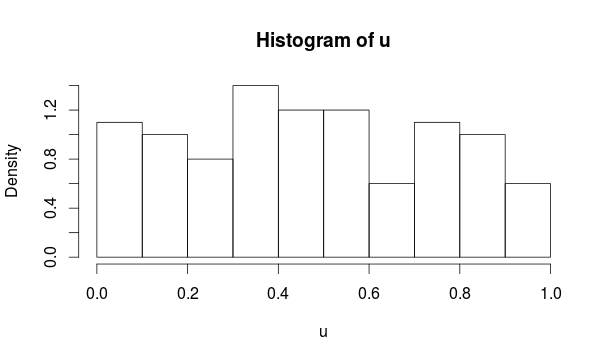
\includegraphics[scale=0.5]{img/histogram_u}\centering
	\caption{Histogram náhodného rozdělení.}
	\label{obr:histogram_u}
\end{figure}

\subsubsection{Histogram exponenciálního rozdělení}
  \begin{lstlisting}[frame=single]  % Start your code-block
  	
hist(x, breaks=5*K, freq=FALSE)
xGrid=seq(min(x)-0.2*xWidth,max(x)+0.2*xWidth,length=n) 
lines (xGrid,dexp(xGrid, rate=L), col='red') 
\end{lstlisting}
\begin{figure}[ht!]
	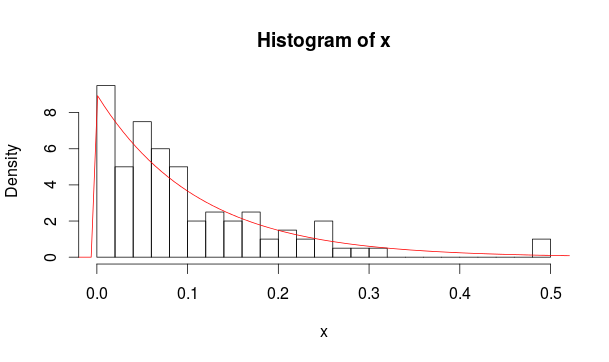
\includegraphics[scale=0.5]{img/histogram_x}\centering
	\caption{Histogram náhodného rozdělení.}
 	\label{obr:histogram_x}
\end{figure}

\subsection{Graf empirické distribuční funkce}
  \begin{lstlisting}[frame=single]  % Start your code-block
  
plot(ecdf(x), verticals=TRUE, do.points = FALSE)
lines (xGrid,pexp(xGrid, rate = L), col='red')
\end{lstlisting}
\begin{figure}[ht!]
	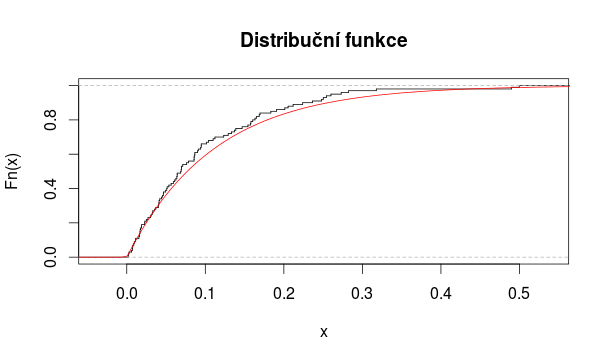
\includegraphics[scale=0.5]{img/1_3empiricka_distribucni_funkce}\centering
	\caption{Graf empirické distribuční funkce spolu s grafem Exp(L)}
	\label{obr:sikme}
\end{figure}

\subsection{Generování pravděpodobnostního papíru}
  \begin{lstlisting}[frame=single]  % Start your code-block
  
y=rexp(n, rate=L)
qqplot(x, y)
abline(0,1, col='red', lwd=2)
\end{lstlisting}
\begin{figure}[ht!]
	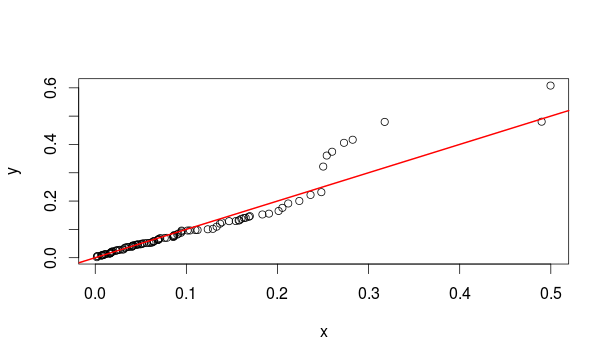
\includegraphics[scale=0.5]{img/1_4_pravdepodobnostni_papir}\centering
	\caption{Porovnání dat x s rozdělením Exp(L)}
	\label{obr:sikme}
\end{figure}

\subsection{Diskuze kvality vygenerovaných dat}
\begin{footnotesize}
\color{black}
Vygenerovaná náhodná data \textcolor{red}{u} se dle histogramu na obrázku \ref{obr:histogram_u} zdají být rovnoměrná.

Histogram z obrázku \ref{obr:histogram_x} nám potvrzuje, že i data \textcolor{red}{x} jsme vygenerovali z náhodných hodnot exponencionálního
rozdělení správně. To nám potvrzuje.

\textcolor{red}{TODO: POPSAT GRAF EMPIRICKE FCE}

\textcolor{red}{TODO: VĚTA PŘÍLIŠ NEZAPADÁ DO KONTEXTU}
V tomto konkrétním případě lze na pravděpodobnostním papíře pozorovat velké rozdíly v datech u hodnot vetších než $0,26$.
\end{footnotesize}

\subsection{Test dobé shody}
Vstup:
 \begin{lstlisting}[frame=single]  % Start your code-block
  
chisq.test(x, p=y/sum(y)) 
\end{lstlisting}
Výstup
 \begin{lstlisting}[frame=single]  % Start your code-block
  
data:  x
X-squared = %* \textcolor{red} {57.6125}, df = 99, p-value = 0.9997
\end{lstlisting}
%%%%%%%%%%%%%%%%%%%%%%%%%%%%%%%%%%%%%%%%%%%%%%%%%%%%%%%%%%%%%%%%%%%%%%%%%%%%

\section{Generování nehomogenního Poissonova procesu}
\subsection{Intenzita příchodů požadavků na server}
 \begin{lstlisting}[frame=single]  % Start your code-block
  
lambda = function(t){100+50*exp(-(t-420)^2/(3600*L))+100*
                       exp(-(L*(-30*L+t-480)^2)/360000)}
# prvni perioda
t=seq(0,3*(24*60)-1)
plot(t,lambda(t%%(24*60)),lty="solid",lwd=3,type='l',
     main="Intenzita přístupů za den",
     ylab="Příchody za minutu",
     xlab="Čas t v minutách")
text(0, 200, "Den 1", cex=0.6, pos=4)
text(24*60, 200, "Den 2", cex=0.6, pos=4)
text(24*120, 200, "Den 3", cex=0.6, pos=4)
abline(h = 0, v = 01)
abline(h = 0, v = 24*60)
abline(h = 0, v = 24*120)
\end{lstlisting}
\begin{figure}[ht!]
	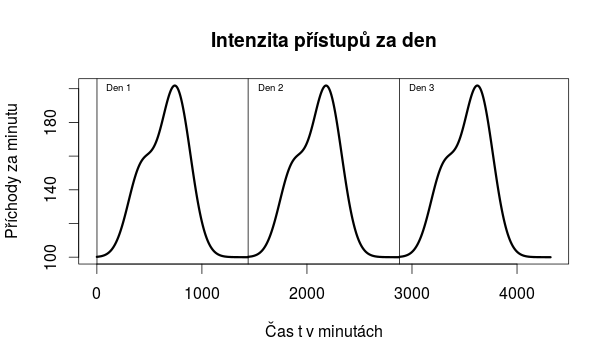
\includegraphics[scale=0.5]{img/2_1_intenzita_prichodu}\centering
	\caption{Intenzita příchodů požadavků na server za tři dny}
	\label{obr:sikme}
\end{figure}

\subsection{Generovánní časů příchodů}
 \begin{lstlisting}[frame=single]  % Start your code-block
  
p = K*10 # prichod
event = numeric(p)
s = 10^-(2.4) # step
t = 0 # time = Aktuální cas
i = p # iterator

# Cyklus simuluje ubíhající čas (po skocích delta) a na základe
# funkce lambda generuje příchod zákazníka
while (0 < i) {
  if (runif(1, min=0, max=1) < lambda(t) * s) {
    i = i - 1
    event[i] = t # oznacime cas udalosti
  }
  t = t + s
} 
plot(event, numeric(p))
\end{lstlisting}
\begin{figure}[ht!]
	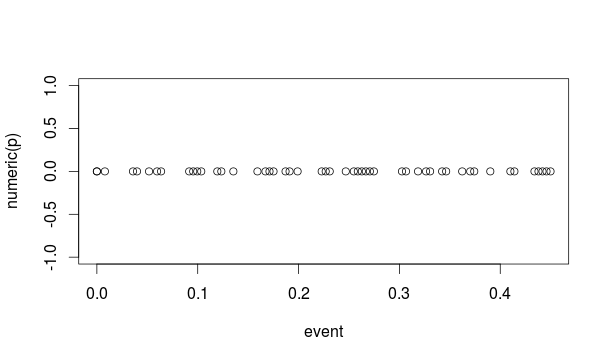
\includegraphics[scale=0.5]{img/2_2_casy_prichodu}\centering
	\caption{Vygenerované časy příchodů.}
	\label{obr:sikme}
\end{figure}

\subsection{Zobrazení četnosti příchodů}
 \begin{lstlisting}[frame=single]  % Start your code-block
  
Zatim nic
\end{lstlisting}
\begin{figure}[ht!]
	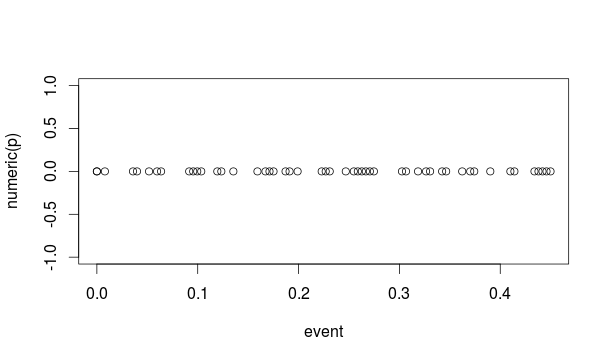
\includegraphics[scale=0.5]{img/2_2_casy_prichodu}\centering
	\caption{Vygenerované časy příchodů.}
	\label{obr:sikme}
\end{figure}
\subsection{Diskuze kvality vygenerovaných dat}

%%%%%%%%%%%%%%%%%%%%%%%%%%%%%%%%%%%%%%%%%%%%%%%%%%%%%%%%%%%%%%%%%%%%%%%%%%%%
%%%%%%%%%%%%%%%%%%%%%%%%%%%%%%%%%%%%%%%%%%%%%%%%%%%%%%%%%%%%%%%%%%%%%%%%%%%%
%%%%%%%%%%%%%%%%%%%%%%%%%%%%%%%%%%%%%%%%%%%%%%%%%%%%%%%%%%%%%%%%%%%%%%%%%%%%
%%%%%%%%%%%%%%%%%%%%%%%%%%%%%%%%%%%%%%%%%%%%%%%%%%%%%%%%%%%%%%%%%%%%%%%%%%%%
%%%%%%%%%%%%%%%%%%%%%%%%%%%%%%%%%%%%%%%%%%%%%%%%%%%%%%%%%%%%%%%%%%%%%%%%%%%%
%%%%%%%%%%%%%%%%%%%%%%%%%%%%%%%%%%%%%%%%%%%%%%%%%%%%%%%%%%%%%%%%%%%%%%%%%%%%
\section{ Simulace internetového obchodu s tokem nákupů dle nehomogenního Poissonova procesu}
\subsection{Intenzita příchodů požadavků na server}
\begin{lstlisting}[frame=single]  % start your code-block

vezme_kuryra=K/(K+L)  # Ze všech zákazníků K/(K+L) použije kurýrní službu
za_minutu_kuryr=numeric(day) 
# Cyklus prochází všechny minutové výskyty a spočíta pravděpodobnosti,
# že zákazník použije kurýra
m=day
while (0 < m) { # pro kazdou minutu po cely den
  o=cetnosti_za_minutu[m] # pocet objednavek za minutu m
  while(0<o){ # pro vsechny objednavky za tu minutu
    if(runif(1,min=0,max=1)<vezme_kuryra){ # zvoli kuryra?
      `+`(za_minutu_kuryr[m])<-1
    }
    `-`(o)<-1
  }
  `-`(m)<-1
}
za_minutu_posta=cetnosti_za_minutu-za_minutu_kuryr
plot(day_seq,za_minutu_kuryr,lwd=1,col='lightgreen',type='l',
     ylim=c(10,150),
     main="Způsoby dodávky",
     ylab="Četnosti příchodů objednávek",
     xlab="Čas t v minutách")
lines(day_seq,lamda_day_seq*vezme_kuryra,lwd=3,col='green')
lines(day_seq,za_minutu_posta,lwd=1, col='lightpink',type='l')
# pravdepodovnost, ze vezmou postu je doplnkem k tomu,
# ze vezmou kuryra
lines(day_seq,lamda_day_seq*(1-vezme_kuryra),lwd=3,col='red')
legend(x=1200,y=150,c("kurýr","pošta"),cex=.8, 
       col=c("green","red"),lty=c(1,1))
\end{lstlisting}
\begin{figure}[ht!]
	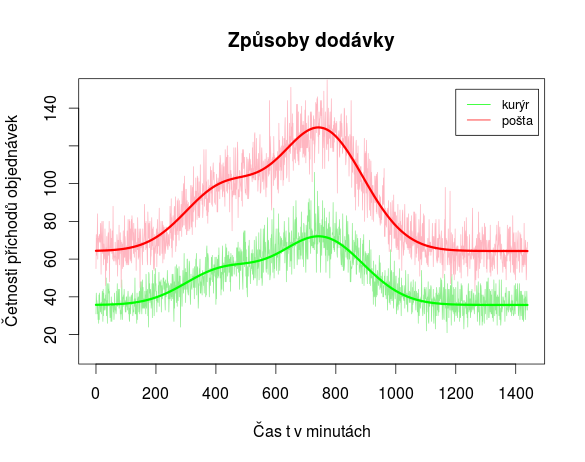
\includegraphics[scale=0.6]{img/3_zpusoby_dodavky}\centering
	\caption{Způsoby dodávky za den}
	\label{obr:sikme}
\end{figure}

\begin{thebibliography}{1}

\bibitem{wiki}
Exponential distribution. In: \textit{Wikipedia: the free encyclopedia} [online]. San Francisco (CA): Wikimedia Foundation, 2001- [cit. 2015-04-21]. Dostupné z: \url{http://en.wikipedia.org/wiki/Exponential_distribution\#Generating_exponential_variates}

\end{thebibliography}

\end{document}
